\documentclass{article} % For LaTeX2e
\usepackage{iclr2019_conference,times}

% Optional math commands from https://github.com/goodfeli/dlbook_notation.
%\input{math_commands.tex}


\usepackage[utf8]{inputenc} % allow utf-8 input
\usepackage[T1]{fontenc}    % use 8-bit T1 fonts
\usepackage{hyperref}       % hyperlinks
\usepackage{url}            % simple URL typesetting
\usepackage{booktabs}       % professional-quality tables
\usepackage{amsfonts}       % blackboard math symbols
\usepackage{nicefrac}       % compact symbols for 1/2, etc.
\usepackage{microtype}      % microtypography

\usepackage{placeins}

\usepackage{hyperref}

\usepackage{amssymb}
\usepackage{amsmath}

% For citations
%\usepackage[numbers, sort&compress]{natbib}
%\usepackage[numbers]{natbib}
%\usepackage{natbib}

% For figures
\usepackage{graphicx} % more modern
\usepackage{wrapfig}
%\usepackage{epsfig} % less modern
%\usepackage{subfigure} 
\usepackage{subcaption} 
\usepackage{multirow}
\usepackage{adjustbox}

\usepackage{listings}
\usepackage{textcomp}

% For assumptions
\usepackage{amsthm,amssymb,amsopn}
\newtheorem{assumption}{Assumption}
\newtheorem{define}{Definition}
\newtheorem{thm}{Theorem}
\newtheorem{lem}{Lemma}
\newtheorem{coro}{Corollary}
\newtheorem{condition}{Condition}
\usepackage{xspace}
\usepackage{bm}

% For algorithms
\usepackage{algorithm}
\usepackage{algorithmic}
\renewcommand{\algorithmiccomment}[1]{~~~~\textcolor{gray}{$\triangleright$\textit{#1}}}
\renewcommand{\algorithmicrequire}{\textbf{Input:}}
\renewcommand{\algorithmicensure}{\textbf{Output:}}
\makeatletter
\makeatletter
\newcommand*{\da@rightarrow}{\mathchar"0\hexnumber@\symAMSa 4B }
\newcommand*{\da@leftarrow}{\mathchar"0\hexnumber@\symAMSa 4C }
\newcommand*{\xdashrightarrow}[2][]{%
  \mathrel{%
    \mathpalette{\da@xarrow{#1}{#2}{}\da@rightarrow{\,}{}}{}%
  }%
}
\newcommand{\xdashleftarrow}[2][]{%
  \mathrel{%
    \mathpalette{\da@xarrow{#1}{#2}\da@leftarrow{}{}{\,}}{}%
  }%
}
\newcommand*{\da@xarrow}[7]{%
  % #1: below
  % #2: above
  % #3: arrow left
  % #4: arrow right
  % #5: space left 
  % #6: space right
  % #7: math style 
  \sbox0{$\ifx#7\scriptstyle\scriptscriptstyle\else\scriptstyle\fi#5#1#6\m@th$}%
  \sbox2{$\ifx#7\scriptstyle\scriptscriptstyle\else\scriptstyle\fi#5#2#6\m@th$}%
  \sbox4{$#7\dabar@\m@th$}%
  \dimen@=\wd0 %
  \ifdim\wd2 >\dimen@
    \dimen@=\wd2 %   
  \fi
  \count@=2 %
  \def\da@bars{\dabar@\dabar@}%
  \@whiledim\count@\wd4<\dimen@\do{%
    \advance\count@\@ne
    \expandafter\def\expandafter\da@bars\expandafter{%
      \da@bars
      \dabar@ 
    }%
  }%  
  \mathrel{#3}%
  \mathrel{%   
    \mathop{\da@bars}\limits
    \ifx\\#1\\%
    \else
      _{\copy0}%
    \fi
    \ifx\\#2\\%
    \else
      ^{\copy2}%
    \fi
  }%   
  \mathrel{#4}%
}
\makeatother

% for striking out.
%\usepackage[normalem]{ulem}

%% For highlighting any changes
%\usepackage{changes}
%\definechangesauthor[name={jab}, color=orange]{jab}

\title{A Generative Model for Electron Paths}

% The \author macro works with any number of authors. There are two
% commands used to separate the names and addresses of multiple
% authors: \And and \AND.
%
% Using \And between authors leaves it to LaTeX to determine where to
% break the lines. Using \AND forces a line break at that point. So,
% if LaTeX puts 3 of 4 authors names on the first line, and the last
% on the second line, try using \AND instead of \And before the third
% author name.




\author{John Bradshaw \\ 
University of Cambridge \\
Max Planck Institute, T\"ubingen 
\\
\texttt{jab255@cam.ac.uk}
\And
Matt J. Kusner \\
University of Oxford \\
Alan Turing Institute
\\
\texttt{mkusner@turing.ac.uk}
\And
Brooks Paige \\
Alan Turing Institute \\
University of Cambridge 
\\
\texttt{bpaige@turing.ac.uk}
\AND
Marwin H. S. Segler \\
BenevolentAI \\
\texttt{marwin.segler@benevolent.ai}
\And
Jos\'e Miguel Hern\'andez-Lobato \\
University of Cambridge \\
Microsoft Research Cambridge \\
Alan Turing Institute \\
\texttt{jmh233@cam.ac.uk}
}


\newcommand{\xb}{\mathbf{x}}
\newcommand{\Xc}{\mathcal{X}}
\newcommand{\Zc}{{\mathcal{Z}}}
\newcommand{\Mc}{{\mathcal{M}}}
\newcommand{\Bc}{{\mathcal{B}}}
\newcommand{\Ac}{{\mathcal{A}}}
\newcommand{\Pc}{{\mathcal{P}}}
\newcommand{\bb}{{\mathbf{b}}}
\newcommand{\ab}{{\mathbf{a}}}
\newcommand{\mb}{{\mathbf{m}}}
\newcommand{\Mb}{{\mathbf{M}}}
\newcommand{\Pb}{{\mathbf{P}}}
\newcommand{\Hb}{{\mathbf{H}}}
\newcommand{\Ab}{{\mathbf{A}}}
\newcommand{\delb}{{\boldmath{\delta}}}



% The model definitions
\newcommand{\electronPath}{\Pc}
\newcommand{\moleculeSet}{\Mc}
\newcommand{\initialAndReactants}{\Mc_0, \Mc_r}


% Then the modules!
\newcommand{\fEmbed}{g_{\Ac}}
\newcommand{\fAdd}{f_{\textrm{add}}}
\newcommand{\fRemove}{f_{\textrm{remove}}}
\newcommand{\fInitial}{f_{\textrm{initial}}}
\newcommand{\fStop}{f_{\textrm{stop}}}
\newcommand{\fReagEmbed}{f_{\textrm{reagent}}}
\newcommand{\fModules}{\fEmbed, \fAdd, \fRemove, \fInitial,\fStop, \fReagEmbed}
\newcommand{\fui}{f_i}
\newcommand{\fuj}{f_j}
\newcommand{\fuk}{f_k}

\newcommand{\actionProb}[2][]{ p(a_{#2} \mid \moleculeSet_{\electronPath_{0:#2-1}^{#1}}, a^{#1}_{#2-1}, #2)}
\newcommand{\continueProb}[2]{p(s_{#1}' \mid \moleculeSet_{#2}) }


% The \author macro works with any number of authors. There are two commands
% used to separate the names and addresses of multiple authors: \And and \AND.
%
% Using \And between authors leaves it to \LaTeX{} to determine where to break
% the lines. Using \AND forces a linebreak at that point. So, if \LaTeX{}
% puts 3 of 4 authors names on the first line, and the last on the second
% line, try using \AND instead of \And before the third author name.

\newcommand{\fix}{\marginpar{FIX}}
\newcommand{\new}{\marginpar{NEW}}

\iclrfinalcopy % Uncomment for camera-ready version, but NOT for submission.
\begin{document}


\maketitle

\begin{abstract}
Chemical reactions can be described as the stepwise redistribution of electrons in molecules. 
As such, reactions are often depicted using ``arrow-pushing'' diagrams which show this movement as a sequence of arrows. 
We propose an electron path prediction model (\ourModel) to learn these sequences directly from data.
Instead of predicting product molecules directly from reactant molecules in one shot, learning a model of electron movement has the benefits of 
(a) being easy for chemists to interpret, 
(b) incorporating constraints of chemistry, such as balanced atom counts before and after the reaction, and 
(c) naturally encoding the sparsity of chemical reactions, which usually involve only a small number of atoms in the reactants.
We design a method to extract approximate reaction paths from any dataset of reaction SMILES strings. %Even though this procedure removes $27\%$ of the USPTO reaction training dataset, 
Our model achieves state-of-the-art results on a subset of the UPSTO reaction dataset. Furthermore, we show that the model recovers a basic knowledge of chemistry without being explicitly trained to do so.
% also it means the sides balance
\end{abstract}



\section{Introduction}
% !TEX root =  ../main_iclr.tex

The ability to reliably predict the products of chemical reactions is of central importance to the manufacture of medicines and materials, and to understand many processes in molecular biology.
Theoretically, all chemical reactions can be described by the stepwise rearrangement of electrons in molecules \citep{herges1994organizing}. 
This sequence of bond-making and breaking is known as the \emph{reaction mechanism}. 
Understanding the reaction mechanism is crucial because it not only determines the products (formed at the last step of the mechanism), 
but it also provides insight into why the products are formed on an atomistic level. 
%
Mechanisms can be treated at different levels of abstraction. 
On the lowest level, quantum-mechanical simulations of the electronic structure can be performed, which is prohibitively computationally expensive for most systems of interest. 
On the other end, chemical reactions can be treated as rules that ``rewrite'' reactant molecules to products, which abstracts away the individual electron redistribution steps into a single, global transformation step. 
To combine the advantages of both approaches, chemists use a powerful qualitative model of quantum chemistry colloquially called ``arrow pushing'', which simplifies the stepwise electron shifts using sequences of arrows which indicate the path of electrons throughout molecular graphs \citep{herges1994organizing}. 

Recently, there have been a number of machine learning models proposed for directly predicting the products of chemical reactions \citep{coley2017prediction,jin2017predicting,schwaller2017found,neural-symbolic,segler2018planning,wei2016neural}, largely using graph-based or machine translation models. 
The task of reaction product prediction is shown on the left-hand side of Figure~\ref{fig:task-overview}. 

In this paper we propose a machine learning model to predict the reaction mechanism, as shown on the right-hand side of Figure~\ref{fig:task-overview}, for a particularly important subset of organic reactions.
We argue that not only is our model more interpretable than product prediction models but it is easier to encode in it the constraints imposed by chemistry. 
Proposed approaches to predicting reaction mechanisms have often been based on combining hand-coded heuristics and quantum mechanics \citep{bergeler2015heuristics,kim2018efficient,nandi2017tabu,rappoport2014complex,simm2017context,zimmerman2013automated}, 
rather than using machine learning.
We call our model \ourModel, as it directly predicts the path of electrons through molecules (i.e., the reaction mechanism). 
To train the model we devise a general technique to obtain approximate reaction mechanisms purely from data about the reactants and products. 
This allows one to train our a model on large, unannotated reaction datasets such as USPTO \cite{lowe2012extraction}. We demonstrate that not only does our model achieve impressive results, surprisingly it also learns chemical properties it was not explicitly trained on.





% \section{Related Work}
% <<<<<<< HEAD
We start by summarizing the related work on \emph{product prediction} and \emph{mechanism prediction} with a particular emphasis on whether the techniques are end-to-end trainable. Table~\ref{table.existing} gives a summary of this section.


\begin{wrapfigure}{R}{0.6\textwidth}
\vspace{-4ex}
\begin{minipage}{0.6\textwidth}
\begin{table}[H]
\begin{tabular}{c|ccc} 
\hline
 \textbf{Prior Work} & \textbf{end-to-end} & \textbf{mechanism}  \\ \hline \hline
\cite{wei2016neural} & \checkmark & $-$  \\ \hline
\cite{coley2017prediction} & $-$ & $-$ \\ \hline
\cite{jin2017predicting} &$-$ &$-$ &  \\ \hline
\cite{schwaller2017found} & \checkmark &$-$  \\ \hline
\cite{segler2017modelling} & \checkmark & $-$ \\ \hline 
\cite{segler2018planning} & \checkmark &$-$  \\ \hline
\cite{NIPS2011_4356} &$-$ & \checkmark  \\ \hline
\cite{kayala2011learning} & $-$ & \checkmark \\ \hline
\cite{kayala2012reactionpredictor} &$-$ & \checkmark  \\ \hline
\cite{fooshee2018deep} & $-$ & \checkmark \\ \hline
\textbf{this work} & \checkmark & \checkmark \\
\hline
%\bf{Method} & %\multicolumn{2}{c}{\bf Full} & \multicolumn{2}{c}{\bf Unaware} & \multicolumn{2}{c}{\bf Fair L2} & \multicolumn{2}{c}{\bf Fair L3} \\
\end{tabular}
\centering
	\caption{Work on machine learning for reaction prediction, and whether they are (a) end-to-end trainable and (b) predict the reaction mechanism. \label{table.existing}}
\end{table}
\end{minipage}
\vspace{-4ex}
\end{wrapfigure}


\paragraph{Product prediction.}

% wei2016neural
% NOTE: Jennifer, David and Alan were not the first to apply deep learning to this problem, this was done Aires de Sousa's group already in 2005, using unsupervised pretraining.
Recently, methods combining machine learning and global rewriting rules have been proposed [\cite{coley2017prediction,neural-symbolic,segler2018planning,wei2016neural,zhang2005structure}]. Here, a learned model is used to predict which rewrite rule to apply preferably. While these models are readily interpretable, they tend be brittle. 
%The earliest work we are aware of that uses deep learning to predict the products of reactions is \cite{zhang2005structure}. Their idea was to approximate the operations of a molecular fingerprint so that all operations become continuously differentiable. They then learned parameters of this fingerprint to accurately predict product fingerprints end-to-end.

% jin2017predicting
Another class of models is the graph-based technique by \cite{jin2017predicting} who construct a network based on the Weisfeiler-Lehman algorithm for testing graph isomorphism. They use this algorithm to select atoms that will be involved in a reaction. They then enumerate all chemically-valid bond changes involving these atoms and learn a separate network to rank the resulting potential products. This method is state-of-the-art on product prediction.

% schwaller2017found
\cite{schwaller2017found} represents reactants as SMILES (CITE) strings and then used a sequence to sequence network (specifically, the work of (CITE)) to predict product SMILES. While this method is end-to-end trainable the SMILES representation is quite brittle as often single character changes will not correspond to a valid molecule.
% segler2017modelling
% TODO
% segler2018planning
% TODO

\paragraph{Mechanism prediction.}
The only other work we are aware of to use machine learning to predict reaction mechanisms are \cite{fooshee2018deep,kayala2012reactionpredictor,NIPS2011_4356,kayala2011learning}.
All of these model a chemical reaction as an interaction between atoms which function as electron donors and those which function as electron acceptors. They predict the reaction mechanism via two independent models: one that identifies these likely electron sources and sinks, and another that ranks all combinations of them.
However, this combining and then ranking of electron sources and sinks can be a slow process, as many plausible reactions need to be considered (the number of subgraphs of $n$ reacting atoms, where single bonds are either added or removed is $2^{n(n-1)/2}$).
These models also have only so far been successfully trained on small hand-curated datasets.
% kayala NIPS: NIPS2011_4356
% kayala2011learning
% kayala2012reactionpredictor
% fooshee2018deep

=======
>>>>>>> master


\section{Background}
% !TEX root =  ../main.tex


\begin{figure*}[t!]
\centering
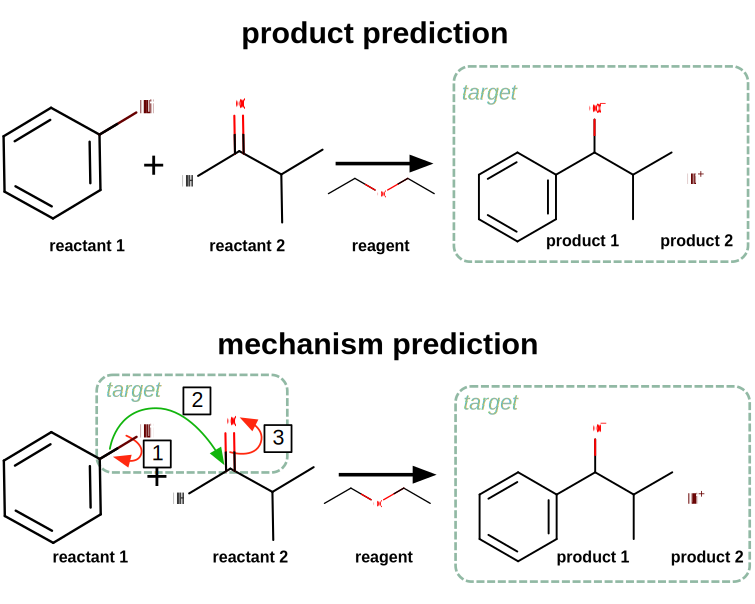
\includegraphics[width=\textwidth]{reaction_diagram}
\caption{\emph{(Left)} The reaction product prediction problem: Given the reactants and reagents, predict the structure of the product. \emph{(Right)} The reaction mechanism prediction problem: Given the reactants, reagents and products, predict how the reaction occurred to form the products.}
\label{fig:task-overview}
%\vspace{-1em}
\end{figure*}


In Figure~\ref{fig:task-overview} we show the two challenges we tackle in this paper. 
On the left we show product prediction; where the goal is to predict the reaction products, given a set of reactants and reagents. However, for this task we do not care {\em how} the reactants react.
 This job of finding the {\em how} is the target of reaction mechanism prediction. 
 %where the steps in a reaction are called a reaction mechanism.
 Before describing how our model predicts mechanisms, we use this section to detail the types of reactions we consider in this paper, and their properties.


%\todo[]{Where is the related work section going...? "And how it relates to previous work on reaction prediction. -- " }

\vspace{-0.15cm}
\paragraph{Molecules and Chemical reactions.}


%In reality, the structure of a molecule is due to how electrons on each atom are interacting with each other. 
%Molecules consist of a set of atoms that are arranged into a structure by bonds, which are localized electrons. 
Molecules can be modeled as a graph structure, where each node is an atom and each edge is a covalent bond.
These covalent bonds represent the fact that 
one or more pairs of electrons are shared between the atoms that the bond connects. 


Just as electrons describe the current structure of molecules, 
they also describe how molecules react with other molecules to produce new ones. All chemical reactions involve the stepwise movement of electrons along the atoms in a set of reactant molecules. 
This movement causes the formation and breaking of chemical bonds that changes the reactants into a new set of product molecules \cite{herges1994coarctate}. Reagent molecules, while helping facilitate the reaction, are not involved in this electron movement.
In this work, we will only consider reactions with steps that involve a single pair of electrons, and
where steps start either with the electron pair on a single atom (called a \emph{lone pair}), or with the electrons in an existing bond. This class of reactions is called \emph{elementary heterolytic reactions}.
These kind of reactions describe more than 80\% of \emph{organic reactions} \cite{herges1994coarctate} 
(reactions outside of this group are homolytic reactions, and electrocyclic reactions).
Organic reactions are those involving carbon atoms, and have a large number of applications from drug design to the invention of new materials \citep{segler2018planning}.

\vspace{-0.15cm}
\paragraph{Reactions as single electron paths.}
If reactions satisfy the above assumptions, then a chemical reaction can be modeled as pairs of electrons moving in a \emph{single path} through the reactant atoms. 
Further, this electron path will alternately remove existing bonds in molecules, and form new ones. We show this alternating structure in the right hand part of Figure \ref{fig:task-overview}. 
The reaction formally starts by taking the pair of electrons between the Li and C atoms and moving them to the C atom (step 1); this is a remove bond step. 
Next comes an add step where electrons are moved from the C atom to form a bond between the two reactant molecules (step 2).
Then a pair of electrons are removed between the C and O atoms and moved to the O atom, giving rise to the products (step 3). 
Predicting the final product is thus a byproduct of predicting this series of electron steps.

However, there are a number of benefits of predicting electron paths over predicting the outcomes of reactions directly (as is done in previous work \cite{jin2017predicting,schwaller2017found}):
\begin{itemize}
\item \textbf{Easy to interpret}: If the model makes a mistake, it is easy to see where, and possibly why, it goes wrong by comparing the steps of the path with the correct steps.
\item \textbf{Sparse}: Reactions often only affect between 3 and 7 atoms out of anywhere from 10-50 reactant atoms. Modeling the reaction as a path allows us to exploit this sparsity.
\item \textbf{Chemical constraints}: Learning a path allows us to easily incorporate chemical constraints, such as the alternating removal and addition of bonds, among others.
% MATT note: not sure I understand this last point
\item \textbf{Compositionally}: Learning to combine lower-level abstractions of chemistry potentially allows us to generalize better.
\end{itemize}
The only other work we are aware of to use machine learning to predict reaction mechanisms are the works \cite{kayala2011learning,kayala2012reactionpredictor}. However,
these rely on complex hand-coded rules and expert-annotated datasets, which are usually small and proprietary.
% Machine learning has been applied mostly for the quantum chemistry-level\cite{NIPS2012_4830,schutt2017schnet}. Additionally, various models have been proposed to predict global rewriting rules for reaction prediction\cite{coley2017prediction,jin2017predicting,neural-symbolic,schwaller2017found,wei2016neural,zhang2005structure}. These models can be trained on large sets of reported chemical reactions. 
%At the medium level of abstraction, Kayala et al. proposed a model to predict electron shift steps using of two independently learned learning-to-rank and scoring stages,
% which however relies on complex hand-coded rules and expert-annotated datasets, which are usually very small.







\section{The Generative Model}

\label{sec:model}
% !TEX root =  ../main_iclr.tex



In this section we define a probabilistic model that describes the movement of electrons that define linear topology reactions.
We represent a set of molecules as a set of graphs $\moleculeSet$, with atoms $\Ac$ as vertices and bonds $\Bc$ as edges;
each connected component of the graph defines an individual molecule.
We can associate an ordering over all the atoms in all the molecules in the set using an {\em atom map} number:
an integer label assigned to each non-hydrogen atom in both the reactants and the products which 
both permits easy matching between atoms before and after the reaction, and
gives us a consistent way to index particular atoms. Molecules input into the model are first put in a Kekul\'e form, a process which makes explicit the location of single and double bonds in aromatic structures;
each bond $b \in \Bc$ is either a single, double, or triple bond.

Each atom $v \in \Ac$ includes a set of features, such as its atom type (e.g. carbon, oxygen, \dots); the full list of input atom features can be found in Table 3 of the appendix.
 However, when learning functions that operate over these atoms we do not work with these raw features directly but instead with the atom, or equivalently node, embedding. 
 These contain information about the atom of interest as well as its surrounding neighborhood.
 These can be computed using any model that is able to compute graph-isomorphic features, for instance usually via message-passing techniques \citep{gilmer2017neural}; we choose to use 4 layer gated graph neural network (GGNN) message functions \citep{li2016gated}, for which we include a short review in the appendix. 
 These produce a $d$-dimensional embedding of an atom and if we stack these vectors up as rows (using the atom mapping to define an order)  we have the matrix $\nodeEmbeddings{\moleculeSet} \subseteq \mathbb{R}^{|\Ac|\times d}$, containing all the node embeddings for a particular molecule set, $\moleculeSet$.

Sometimes we wish to agglomerate the node embeddings belonging to a set of nodes $\Ac'$ (with $\Ac' \subseteq  \Ac$), to form a graph embedding \citet[\S B.1]{li2018learning}, that is a vector that represents multiple nodes but that is invariant to any particular node ordering. 
These functions have also previously been referred to as aggregation graph transformations \citep[\S3]{Johnson2017-pd}.
We denote these functions that map from $\nodeEmbeddings{\moleculeSet'}$ to a $q$-dimensional vector, $r: \mathbb{R}^{|\Ac'|\times d} \to \mathbb{R}^q$.
They obtain their node order invariance by performing a weighted sum over the nodes.


Given an initial set of reactant molecules $\moleculeSet_0$ and a set of reagent molecules $\moleculeSet_r$, 
our model defines a conditional distribution over a sequence of atoms (which we also refer to as actions) $\electronPath_{0:T} = (a_0, a_1, \ldots, a_T)$,
which fully characterizes the electron path.
This electron path in turn deterministically defines both a final product $\moleculeSet_{T+1}$, 
denoting the outcome of the reaction,
as well as a sequence of intermediate products $\moleculeSet_t$, for $t = 1,\dots,T$,
which correspond to the state of the graph after the first $t$ steps in the subsequence $\electronPath_{0:t} = (a_0, \dots, a_t)$ are applied to the initial $\moleculeSet_0$. We also define a stopping sequence $\mathcal{S}_t = (s_0, \ldots, s_{T+1})$ which indicates if the reaction should stop (i.e, $s_t\!=\!1$ if the reaction should stop and is $0$ otherwise). 

We propose to learn a distribution $p_\theta( \electronPath_{0:T} \mid \moleculeSet_0, \moleculeSet_r)$ over electron movements. 
We first detail the generative process %(i.e., the forward pass) 
that specifies $p_\theta$, before describing how to train the model's parameters, $\theta$.


\subsection{Generative process}


\begin{figure*}
\centering
\includegraphics[width=\textwidth]{reaction_model_blue}
\caption{
 This figure shows the sequence of actions in transforming the reactants in box 1 to the products in box 9.
 The sequence of actions will result in a sequence of pairs of atoms, between which bonds will alternately be removed and created, creating a series of intermediate products. 
At each step the model sees the current intermediate product graph (shown in the boxes) as well as the previous action, if applicable, shown by the grey circle. It uses this to decide on the next action.
We represent the characteristic probabilities the model may have over these next actions as colored circles over each atom.
Some actions are disallowed on certain steps, for instance you cannot remove a bond that does not exist; these blocked actions are shown as red crosses.
}
\label{fig:reaction_model}
\end{figure*}







First note that since our reactions are a single path of electrons through the reactants then, at any point, the next step in the path depends only on (i) the intermediate molecule formed by the action path up to that point, (ii) the previous action taken (indicating where the free pair of electrons are) and (iii) the point of time through the path, indicating whether we are on an add or remove bond step. 
We make the simplifying assumption that the stop probability and the actions after the initial action $a_0$ do not depend on the reagents. This leads to a parameterized model with dependency structure:
\begin{align}
\label{eq:jointprob}
p_\theta(\electronPath_{0:T} \mid \moleculeSet_0, \moleculeSet_r) 
&=
	p_\theta(s'_0 \mid \moleculeSet_0)
	p_\theta(a_0 \mid \moleculeSet_0, \moleculeSet_r)\\ \nonumber &\quad \times
	\left[\prod_{t=1}^{T}
		p_\theta(s_{t}' \mid \moleculeSet_{t})
		p_\theta(a_t \mid \moleculeSet_{t}, a_{t-1}, t)
	\right]
	p_\theta(s_{T+1} \mid \moleculeSet_{T+1})
	,
\end{align}
where we have defined $p_\theta(s'_t \mid \moleculeSet_t) \equiv 1 - p_\theta(s_t \mid \moleculeSet_t)$ to be the probability of {\em continuing} a reaction given the current molecule set $\moleculeSet_t$.
The other terms include $p_\theta(a_0 \mid \initialAndReactants)$, the probability of the initial state $a_0$ given the reactants and reagents; 
the conditional probability $p_\theta(a_t \mid  \moleculeSet_t, a_{t-1}, t)$ 
%\todo[]{maybe somehow refer to "bond type" instead of $t$?} 
of next state $a_t$ given the intermediate products $\moleculeSet_t$ for $t > 0$;
and the probability $p_\theta(s_t \mid \moleculeSet_t)$ that the reaction terminates with final product $\moleculeSet_{t}$.


\begin{algorithm}[t]
  \caption{The generative steps of ELECTRO.}
  {\bf Input:}~~Reactant molecules $\Mc_0$ (consisting of atoms $\Ac$), reagents $\Mc_r$, atom embedding function $\fEmbed(\cdot)$, graph embedding function $r(\cdot)$, time steps $T^\mathrm{max}$
  
  \begin{algorithmic}[1]
  	\STATE $\nodeEmbeddings{\moleculeSet_0} = \fEmbed(\Mc_0)$ \COMMENT{atom embedding of reactants}
  	\STATE $\contextVect_\mathrm{reagent} = r(\Mc_r)$ \COMMENT{graph embedding of reagents}
  	%\STATE $\actionLogits = $
  	\STATE $p_{\mathrm{start}}(a_t \mid \moleculeSet_0, \moleculeSet_r) = \mbox{softmax}(\fInitial(\nodeEmbeddings{\moleculeSet_0}, \contextVect_\mathrm{reagent}))$ \COMMENT{probability $a_t$ starts the reaction}
  	\STATE $a_{0} \sim p_{\mathrm{start}}(a_t \mid \moleculeSet_0, \moleculeSet_r)$
  	\FOR{$t = 1, \ldots, T^\mathrm{max}$}
  		\STATE $\moleculeSet_t \leftarrow \moleculeSet_{t-1}, a_{t-1}, \ldots, a_{t-1}$ \COMMENT{modify molecules based on previous molecule and action}
  		\IF{$t \mod 2 = 1$}
  			\STATE a
  		\ENDIF
  		\STATE a
  		%\STATE \mathbf{h}_
  	\ENDFOR
 %  	% Set up pool of completed paths to sort later
 %  	\STATE $\outputPool = \{\left( \emptyset, \log (1 - \cProbCont(\Mc_0)) \right) \}$  \COMMENT{This set will store all completed paths.}
 %  	\STATE $\removeFlag \!=\!1$ \COMMENT{Remove flag}
  	
 %  	% Pick the first action.\\
 %  	\STATE
	% \STATE $\hat{\Bc} = \emptyset$.  \COMMENT{This set will store all possible open paths. Cleared at start of each timestep.}	
	% \FORALL{$v \in \Ac$} 
	% 	\STATE $ \cPath = (v)$
	% 	\STATE $ \lProb = \log \cProbCont(\Mc_0) + \log \cProbInitial(v, \moleculeSet_0, \moleculeSet_r)$
	% 	\STATE $\hat{\Bc} = \hat{\Bc} \cup \{\left(\cPath, \lProb \right)\}$
	% \ENDFOR
	% \STATE  $\Bc_{0} = \texttt{pick\_topK\_actions}(\hat{\Bc})$ \COMMENT{We filter down to the top K most promising actions.}
	
	% % Then we evaluate the next stages.
	% \STATE
	% \FOR{t in $(1, \ldots, T^\mathrm{max})$}
	% 	\STATE $\hat{\Bc} = \emptyset $ 
				
	% 	% We take all the previous top K open paths from the previous step...
	% 	\FORALL{$(\cPath, \lProb) \in \Bc_{t-1}$} 
			
	% 		% We evaluate their stop probability at that point and add these stopped version to the completed pool.
	% 		\STATE $\Mc_\cPath = \texttt{calc\_intermediate\_mol}(\Mc_0, \cPath)$
	% 		\STATE $p_c = \cProbCont(\Mc_\cPath)$
	% 		\STATE $\hat{\Pc} = \hat{\Pc} \cup \{(\cPath, \lProb + \log (1 - p_c))\}$
			
	% 		% We then see what would happen if we continued and picked another action.
	% 		\FORALL{$v \in \Ac$}
	% 			\STATE $\cPath' = \cPath^\frown (v)$ \COMMENT{New proposed path is concatenation of old path with new node.}

	% 			\STATE $v_{t-1} = $ last element of $\cPath$
	% 			\STATE $\hat{\Bc} = \hat{\Bc} \cup \{(\cPath' , \lProb + \log p_c + \log \cProbAct(v, \Mc_\cPath, v_{t-1}, \removeFlag) )\}$
	% 		\ENDFOR
	% 	\ENDFOR
		
	% 	% We next prune down the search space for next iteration to our beam width.
	% 	\STATE  $\Bc_{t} = \texttt{pick\_topK\_actions}(\hat{\Bc})$ 
		
	% 	% We indicate that the next step will be opposite step:
	% 	\STATE $\removeFlag = \removeFlag + 1 \mod 2$. \COMMENT{If on add step change to remove and vice versa.}
	% \ENDFOR
	
 %  % Finally we sort the pool and we are done
 %  \STATE
 %  \STATE $\outputPool = \texttt{sort\_on\_prob}(\outputPool)$
  \end{algorithmic}
  {\bf Output:}~~Valid completed paths and their respective probabilities, sorted by the latter, 
  \label{algo:valid_path}
\end{algorithm}


It is possible to stop prior to selecting a first atom $a_0$, indicating that no reaction would take place.
However, we restrict our model to not stop at step $t\!=\!1$, as it is necessary to pick up a complete electron pair. 
Given any particular selected atom $a_t$ which extends the reaction path, we can deterministically update the previous molecular graph $\moleculeSet_{t}$ to produce the next set of (intermediate) products $\moleculeSet_{t+1}$.

Given our reaction assumptions, then, as stated earlier, there are two types of electron movements that alternate: 
(i) movement that \emph{removes an existing bond}, and 
(ii) movement that \emph{adds a new bond}. 
We define atoms with free electrons as having a self-bond.
Thus, all reactions start by first selecting an atom, removing a bond (between two different atoms, or a self-bond), and then alternately adding and removing bonds;
we can determine whether a particular step is an add step or a remove step by inspecting $t$.
Note that $\moleculeSet_1 = \moleculeSet_0$, as the initial action of selecting $a_0$ does not form or remove any bonds.
Figure~\ref{fig:reaction_model} presents a simple example reaction which demonstrates all the critical features of the model;
the subfigures show the sequence of intermediate products and the distributions over actions.



We are left now with defining the functional form of our conditional distributions in  Eq.~\eqref{eq:jointprob} for continuing $p_\theta(s'_t \mid \moleculeSet_t)$, picking the initial action $p_\theta(a_0 \mid \initialAndReactants)$, and picking subsequent actions $p_\theta(a_t~|~\moleculeSet_t, a_{t-1}, t)$, all of which are parameterized by neural networks.
At each step of the electron path, the network takes the current intermediate graphs, 
the previous action, and the reagents if relevant, 
and computes a probability distribution over next possible actions (i.e., selecting a particular atom, or stopping).
The structure of these networks is described in the following section, although we defer full architectural details (e.g.\ number of layers and hidden units) 
and training settings to the appendix.








\subsection{Computing probabilities over actions}

We now define each of our parameterized distributions over actions.
The simplest of these is $p_\theta(s'_t \mid \moleculeSet_t)$, which is the probability of continuing given the set of intermediate products at time $t$. 
This probability is computed from a graph embedding via the function $\fEmbedGraphs_{\textrm{stop}}$, which projects down to a single dimension. We then map this to the $[0,1]$ interval via the sigmoid function $\sigma$ which yields the overall expression
\begin{align}
%$
p_\theta(s'_t \mid \moleculeSet_t) = \sigma(\fEmbedGraphs_{\textrm{stop}}(\nodeEmbeddings{\moleculeSet_t})).
%$
\end{align}
Each of the three parameterized conditional probability distributions for the {\em start}, {\em add} and {\em remove} steps have similar forms, each defining a probability vector over actions.
The transition distribution $p_\theta(a_t \mid  \moleculeSet_t, a_{t-1}, t)$ 
which selects the next atom in the sequence $\electronPath$
can be split into two distributions depending on the parity of $t$:
the remove bond step distribution $p_\theta^\textrm{remove}(a_t \mid  \moleculeSet_t, a_{t-1})$ is used when $t$ is odd, 
and the add bond step distribution $p_\theta^\textrm{add}(a_t \mid \moleculeSet_t, a_{t-1})$ is used when $t$ is even. 

These three modules each have the same overall functional form
\begin{align}
\actionLogits &= f(\nodeEmbeddings{\moleculeSet_t}, \contextVect), \\
p_\theta(a_t \mid \cdots) &\propto \bm{\beta} \odot \mbox{softmax}(\bm{\actionLogits})
\end{align}
where $f$ is one of the networks $\fInitial, \fAdd$, or $\fRemove$; 
$\contextVect$ is a context vector, and $\bm{\beta}$ is a binary mask.

Each of the three actions has a different context and mask.
The add step $p_\theta^\textrm{add}(a_t \mid \moleculeSet_t, a_{t-1})$ and remove step $p_\theta^\textrm{remove}(a_t \mid \moleculeSet_t, a_{t-1})$,
 have as context the node embedding of the atom selected at the previous step, $\contextVect_{a_{t-1}} = \nodeEmbeddings{\moleculeSet_t, a_{t-1}}$. 
For the initial step, this context vector $\contextVect_\mathrm{reagent}$ is an embedding of all the reagents present, computed 
by a graph embedding function $\fEmbedGraphs_\mathrm{reagent}$.
When computing the output probabilities,
we use the binary vector $\bm{\beta}$ to mask out specific actions known to be impossible.
The value of this differs for the {\em start}, {\em add} and {\em remove} steps;
for the start step any action can be picked, so $\bm{\beta}$ is the all-ones vector.
For the remove step, $\bm{\beta}_\mathrm{remove}$ masks out (i.e.\ is set to zero for) any bonds that do not currently exist and thus cannot be removed (noting though that self-bonds are permitted in the first remove step).
For the add step, $\bm{\beta}_\textrm{add}$ only masks out the previous action, preventing the model from stalling in the same state for multiple time-steps. 
\paragraph{Training}
We can learn the parameters $\theta$ of all the parameterized functions, including those producing node embeddings, by maximizing the log likelihood of a full path $\log p_\theta(\electronPath_{0:T} \mid \moleculeSet_0, \moleculeSet_r)$.
This is evaluated by using a known electron path $a_t^\star$ and intermediate products $\moleculeSet_t^\star$ extracted from training data,
rather than on simulated values. 
This allows us to train on all stages of the reaction at once, given electron path data.
We train our models using Adam \citep{kingma2014adam} and an initial learning rate of $10^{-4}$,
with minibatches of size one, where minibatches often consist of multiple intermediate graphs.

\paragraph{Prediction}
Once trained, we can use our model to sample chemically-valid paths given an input set of reactants $\moleculeSet_0$ and reagents $\moleculeSet_r$, 
simply by simulating from the conditional distributions until sampling a stop value $s_t$.
We instead would like to find a ranked list of the top-$K$ predicted paths, and do so using a modified beam search,
in which we roll out a beam of width $K$ until a maximum path length $T^\mathrm{max}$,
while recording all paths which have terminated.
This search procedure is described in detail in Algorithm 1 in the Appendix.







\section{Reaction Mechanism Identification}

% !TEX root =  ../main.tex

\subsection{Data and preprocessing}

todos:
\begin{itemize}
\item describe dataset
\item describe path extraction
\item describe reagent filtering
\end{itemize}



\section{Experiments and Evaluation}
% !TEX root =  ../main_iclr.tex



\begin{table}[h]%
\begin{minipage}[l]{0.4\textwidth}

\centering
\includegraphics[width=1.\textwidth]{imgs/main_text_input}
\captionof{figure}{
An example of the paths suggested by \ourModelIR on one of the USPTO test examples. Its first choice in this instance is correct.
}
\label{fig:predicted-paths}
 \end{minipage}\hfill%
\begin{minipage}[r]{0.53\textwidth}
%  \centering
  \begin{tabular}{lllll}
    \toprule
    & \multicolumn{4}{c}{Accuracies (\%)}                   \\
    \cmidrule(r){2-5}
    Model Name & Top-1 & Top-2 & Top-3 & Top-5 \\
    \midrule
    \ourModelIR &  70.3 &  82.8 & 87.7 & 92.2    \\
    \ourModelR  &  77.8 &  89.2 & 92.4 & 94.7    \\
    \bottomrule
  \end{tabular}
  \caption{Results when using \ourModel for \emph{mechanism prediction}. Here a prediction is correct if the atom mapped action sequences predicted by our model match exactly those extracted from the USPTO dataset.}
  \label{table:mech-predict}
  \vspace{-0.25cm}
   \end{minipage}

\end{table}

We now evaluate \ourModelR on the task of (i) \emph{mechanism prediction} and (ii) \emph{product prediction} (as described in Figure~\ref{fig:task-overview}). While generally, it is necessary to know the reagents $\moleculeSet_e$ of a reaction to faithfully predict the mechanism and product, it is often possible to make inferences from the reactants alone. Therefore, we trained a second version of our model that we call \ourModelIR, which ignores reagent information. This allows us 
% when selecting the initial action (i.e.\ no context vector $\contextVect_\mathrm{reagent}$ is input into $\fInitial$), 
%allowing 
to gauge the importance of reagents in determining the mechanism of the reaction. %. We now evaluate our model on the \emph{reaction mechanism prediction} and \emph{reaction product prediction} problems.



% In our experiments we consider two variants of our model: 
% the first model \ourModelR  is exactly as defined in Section\ \ref{sec:model}, including all reagent information. 

% While generally all reagents are required to faithfully predict the mechanism and product, it is often possible to makes inferences from the reactants alone. Therefore, we investigated a second version we call \ourModelIR ignores the reagents when selecting the initial action (i.e.\ no context vector $\contextVect_\mathrm{reagent}$ is input into $\fInitial$), 
% allowing us to gauge the importance of reagents in determining what reaction occurs. We now evaluate our model on the \emph{reaction mechanism prediction} and \emph{reaction product prediction} problems.

\subsection{Reaction Mechanism Prediction}

For mechanism prediction we are interested in ensuring we obtain the exact sequence of electron steps correctly. 
%For instance, when forming a bond between two pairs of atoms we want to know which one of the atoms donated the electron pair needed to form the bond, even if the end result is the same. 
%The representation of the reaction mechanism produced by our model is a sequence of atoms, detailing the path taken by the electrons in a series of alternating steps in which bonds are broken and formed; using the atom mapping from the USPTO dataset this takes the form of a series of integers.
We evaluate accuracy by checking whether the sequence of integers extracted from the raw data as described in Section 4
is an exact match with the sequence of integers output by \ourModel. We compute the top-1, top-2, top-3, and top-5 accuracies and shown them in Table \ref{table:mech-predict}, with an example prediction shown in Figure \ref{fig:predicted-paths}.



\subsection{Reaction Product Prediction}
\label{sec:product-prediction}



\begin{table}[t]
%\begin{minipage}[l]{0.42\textwidth}
\begin{center}
  
  %\end{minipage}\hfill
  %\begin{minipage}[r]{0.53\textwidth}
%  \centering
  \begin{tabular}{lllll}
    \toprule
    & \multicolumn{4}{c}{Accuracies (\%)}                   \\
    \cmidrule(r){2-5}
    Model Name & Top-1 & Top-2 & Top-3 & Top-5 \\
    \midrule
    WLDN FTS \citep{jin2017predicting} & 84.0  & 89.2 &  91.1 & 92.3 \\
    WLDN \citep{jin2017predicting} & 83.1 & 89.3 & 91.5 & 92.7 \\
    Seq2Seq FTS \citep{schwaller2017found} & 81.7 & 86.8 & 88.4 & 89.8 \\
    Seq2Seq \citep{schwaller2017found} & 82.6 & 87.3 & 88.8 & 90.1\\
    \bottomrule \toprule
    \ourModelIR &  78.2 & 87.7 & 91.5 & 94.4   \\
    \ourModelR  &  {\bf 87.0} & {\bf 92.6} & {\bf 94.5} & {\bf 95.9}    \\
    \bottomrule
  \end{tabular}
   \caption{Results for \emph{product prediction}, following the product matching procedure in Section~\ref{sec:product-prediction}. 
 For the baselines we compare against models trained (a) on the full USPTO training set (marked FTS) and only tested on our subset of LEF reactions, and (b) those that are also trained on the same subset as our model. 
 We make use of the code and pre-trained models provided by \citet{jin2017predicting}. For the Seq2Seq approach, as neither code nor more fine grained results are available, we train up the required models from scratch using the OpenNMT library \citep{2017opennmt}.
} \label{table:prod-predict}
  %\end{minipage}
    \vspace{-0.25cm}
    \end{center}
\end{table}


Reaction mechanism prediction is useful to ensure we form the correct product in the {\em correct way}.
However, it underestimates the model's actual predictive accuracy: although a single atom mapping is provided as part of the USPTO dataset, in general atom mappings are not unique (e.g., if a molecule contains symmetries). Specifically, multiple different sequences of integers could correspond to chemically-identical electron paths. 
The first figure in the Appendix shows an example of a reaction with symmetries, where different electron paths produce the exact same product. 

Recent approaches to {\em product prediction} \citep{jin2017predicting,schwaller2017found}
have evaluated whether the major product reported in the test dataset matches predicted candidate products generated by their system, independent of mechanism.
In our case, the top-5 accuracy for a particular reaction may include multiple different electron paths that ultimately yield the same product molecule.

To evaluate if our model predicts the same major product as the one in the training data need to solve a graph isomorphism problem. To approximate this 
%Identifying whether two product molecules are chemically the same is equivalent to solving a graph isomorphism over the atoms and bond types, comparing the output of our system to the product molecule.
%To perform this comparison, 
we (a) take the predicted electron path, 
%sequence of edits on the reactants graph defined by an electron path,  
(b) apply these edits to the reactants to produce a product graph (balancing charge to satisfy valence constraints), 
(c) remove atom mappings,
and (d) convert the product graph to a canonical SMILES string representation in Kekul\'e form (aromatic bonds are explicitly represented as double-bonds). 
%then applying the sequence of edits to the reactants graph,
%setting explicit charges or hydrogen counts on the first and last atom in the electron path in order to satisfy valence constraints.
%We then strip all atom map numbers from the graph.
%We can use RDKit to express the molecule in a canonical SMILES string format 
%(predicted electron paths which yield chemically infeasible products are considered failures).
We can then evaluate whether a predicted electron path matches the ground truth by a string comparison. This procedure is inspired by the evaluation of \citet{schwaller2017found}. To obtain a ranked list of products for our model, we compute this canonicalized product SMILES for each of the predictions found by beam search over electron paths, removing duplicates along the way. 
These product-level accuracies are reported in Table \ref{table:prod-predict}.

We compare with the state-of-the-art graph-based method \cite{jin2017predicting};
we use their evaluation code and pre-trained model\footnote{\url{https://github.com/wengong-jin/nips17-rexgen}},
re-evaluated on our extracted test set. 
We also use their code and re-train a model on our extracted training set, to ensure that any differences between our method and theirs is not due to a specialized training task. We also compare against the Seq2Seq model proposed by \citep{schwaller2017found}; 
however, as no code is provided by \citet{schwaller2017found}, we run our own implementation of this method based on the OpenNMT library \citep{2017opennmt}.
Overall, \ourModelR outperforms all other approaches on this task, with 87\% top-1 accuracy and 95.9\% top-5 accuracy.
Omitting the reagents in \ourModelR degrades top-1 accuracy slightly, but maintains a high top-3 and top-5 accuracy,
suggesting that reagent information is necessary to provide context in disambiguating plausible reaction paths.



% If the ultimate desired goal is to predict the product molecule rather than the reaction mechanism,
% a benefit of our approach is the predicted electron paths can then serve as an explanation. 
% In this manner, when showing predicted products, we can list, alongside the maximum likelihood path, any other candidate paths that result in the same product. 







% !TEX root =  ../main.tex

\begin{figure*}[t]

    \centering
    \begin{subfigure}[b]{0.3\textwidth}
        \centering
        \includegraphics[height=0.9in]{imgs/textbook/reaction3}\\\vspace{0.1in}
        %\caption{}
    \end{subfigure}%
    \hspace{1cm}
     \begin{subfigure}[b]{0.5\textwidth}
        \centering
        \includegraphics[height=1.1in]{imgs/textbook/reaction7}
        %\caption{}
    \end{subfigure}
%    \vspace{-1em}
	\caption{(left) 2nd-order nucleophilic substitutions $S_N 2$-reactions, (right) Suzuki-coupling (please note that in the "real" mechanism of the Suzuki coupling, the reaction would proceed via oxidative insertion, transmetallation and reductive elimination at a Palladium catalyst. In this work, we only condition implicitly on catalysts and reagents). In both cases, our model has correctly picked up the trend that halides lower in the period table usually react preferably ($I>Br>Cl$). }
	\label{fig:qualitative}
\vspace{-0.5em}
\end{figure*}



\subsection{Qualitative Analysis}

Complex molecules often feature several potentially reactive functional groups $r=\{F_1,...,F_N\}$, which compete for reaction partners. 
To predict the selectivity, that is which functional group will predominantly react in the presence of other groups, 
students of chemistry learn heuristics and trends, 
which have been established over the course of three centuries of experimental observation.
To qualitatively study whether the model has learned such trends from data we queried the model with several typical text book examples from the chemical curriculum (see Figure \ref{fig:qualitative} and the Appendix). 
We found that the model predicts most examples correctly. In the few incorrect cases, interpreting the model's output reveals that the model made chemically plausible predictions.



\section{Limitations and Future Directions}

In this section we briefly list a couple of limitations of our approach and discuss any pointers towards their resolution in future work.

\paragraph{LEF Topology}

\ourModel can currently only predict reactions with LEF topology (\S \ref{sect:LEF}). 
These are the most common form of reactions \citep{herges1994organizing}, but in future work we would like to extend \ourModel's action repertoire to work with other types of mechanisms such as cyclic or multi-step reactions.
 This could be done by allowing \ourModel to sequentially output a series of paths.
 At training time we would require labelled mechanism paths for these reactions, obtainable from finer grained datasets or perhaps calculated using a QM approach following \citet{Sadowski2016-qg}. 
 
 \paragraph{Graph representation of molecules}

 Although this shortcoming is not just restricted to our work, by modelling molecules and reactions as graphs and operations thereon, we ignore details about the electronic structure and conformational information, ie information about how the molecule shape changes in 3D. 
 This information is crucial in some cases.
 Having said this, there is probably some balance to be struck here, as representing molecules and reactions as graphs is an extremely powerful abstraction, and one that is commonly used by chemists, allowing models working with such graph representations to be more easily interpreted.
 
 


\section{Conclusion}


In this paper we proposed \ourModel, a model for predicting electron paths for reactions with linear electron flow.
These electron paths, or {\em reaction mechanisms}, describe how molecules react together. 
Our model (i) produces output that is easy for chemists to interpret, and (ii) exploits the sparsity and compositionality involved in chemical reactions.
As a byproduct of predicting reaction mechanisms we are also able to perform reaction product prediction,
comparing favorably to the strongest baselines on this task. 
 %Work to extend the model towards all classes of chemical reactions is currently ongoing and will be reported in due course.
%
% \paragraph{Acknowledgements.}
%
%
%
%
%We would like to thank Jennifer Wei, Dennis Sheberla, and David Duvenaud for their very helpful discussions.
%BP and MK are supported by The Alan Turing Institute under the EPSRC grant EP/N510129/1. 
%JB acknowledges support from an EPSRC studentship.



\subsection*{Acknowledgements}

We would like to thank Jennifer Wei, Dennis Sheberla, and David Duvenaud for their very helpful discussions.
This work was supported by The Alan Turing Institute under the EPSRC grant EP/N510129/1. 
JB also acknowledges support from an EPSRC studentship.


%\newpage
\bibliography{bibliography}
%\bibliographystyle{naturemag}
\bibliographystyle{plainnat}

\appendix
\vfill
\pagebreak
\section{Example of symmetry affecting evaluation of electron paths}
In the main text we described the challenges of how to evaluate our model, as different electron paths can form the same products, for instance due to symmetry.
Figure \ref{fig:symmetric-reaction-example} is an example of this.


\begin{figure*}[h]

    \centering
    \begin{subfigure}[b]{0.95\textwidth}
        \centering
        \includegraphics[width=\textwidth]{imgs/symmetry/main_reaction}
        \caption{Reaction as defined by USPTO SMILES}
    \end{subfigure}
    
    \par\bigskip % force a bit of vertical whitespace 
    \begin{subfigure}[b]{0.95\textwidth}
        \centering
        \includegraphics[width=0.4\textwidth]{imgs/symmetry/possible1}
        \qquad
        \qquad
        \includegraphics[width=0.4\textwidth]{imgs/symmetry/possible2}
        \caption{Possible action sequences that all result in same major product.}
    \end{subfigure}
    \caption{This example shows how symmetry can affect the evaluation of electron paths. In this example, although one electron path is given in the USPTO dataset, the initial N that reacts could be either 15 or 12, with no difference in the final product. This is why judging purely based on electron path accuracy can sometimes be misleading.}
    \label{fig:symmetric-reaction-example}
\end{figure*}

\section{Forming Node and Graph Embeddings}

In this section we briefly review existing work for forming node and graph embeddings, as well as describing more specific details relating to our particular implementation of these methods. 
Figure \ref{fig:graph_nn} provides a visualization of these techniques.

\begin{figure*}
\centering
\includegraphics[width=\textwidth]{imgs/graph_nn}
\caption{
Visualization of how node embeddings and graph embeddings are formed. 
Node embeddings are $d$-dimensional vectors, one for each node. 
They are obtained using Gated Graph Neural Networks \citep{li2016gated}.
These networks consist of a series of iterative steps where the embeddings for each node is updated using the node's previous embedding and a message from its neighbors.
 Graph embeddings are $q$-dimensional vectors, representing a set of nodes, which could for instance be all the nodes in a particular graph \citep{li2018learning}.
  They are formed by a weighted sum over node embeddings.
}
\label{fig:graph_nn}
\end{figure*}

 We start with Gated Graph Neural Networks \citep{li2016gated, gilmer2017neural}. 
 We denote these as $\fEmbed: \moleculeSet \to \mathbb{R}^{|\Ac|\times d}$, where we refer to the output as ``node embeddings'', $\nodeEmbeddings{\moleculeSet} \subseteq \mathbb{R}^{|\Ac|\times d}$. 
These networks form these node embeddings through a recurrent operation on messages, $\mb_v$, with $v \in \Ac$ so that there is one message associated with each node.
At the first time step these messages, $\mb_v^{(0)}$, are initialized with the respective atom features shown in Table \ref{table:atom-features}. GGNNs then update these messages in a recursive nature:

\begin{align}
	\mb_v^{(s)} = \textrm{GRU}\left( 
					\mb_v^{(s - 1)},  
						\sum_{i \in \neigh{1}(v)} f_\textrm{single}\left(\mb_i^{(s - 1)}\right) +
						\sum_{j \in \neigh{2}(v)} f_\textrm{double}\left(\mb_j^{(s - 1)}\right) +
						\sum_{k \in \neigh{3}(v)} f_\textrm{triple}\left(\mb_j^{(s - 1)}\right)
					\right)
\end{align}

Where $\textrm{GRU}$ is a Gated Recurrent Unit \citep{Cho2014-xt}, the functions $\neigh{1}(v)$, $\neigh{2}(v)$, $\neigh{3}(v)$ index the nodes connected by single, double and triple bonds to node $v$ respectively and $f_\textrm{single}$, $f_\textrm{double}$ and $f_\textrm{triple}$ are linear transformations with learnable parameters.
This process continues for $S$ steps (where we choose $S=4$), with all the messages and the hidden layer of the GRU maintaining the same dimensionality of 101 as the raw atom features.
The node embeddings are set as the final message belonging to a node, so that indexing a row of the node embeddings matrix, $\nodeEmbeddings{\moleculeSet}$, gives a transpose of the final message vector, ie $[\nodeEmbeddings{\moleculeSet}]_v = \mb_v^{(S)t}$.

\begin{table}
  \caption{Atom features we sue as input to the GGNN. These are calculated using RDKit.}
  \label{table:atom-features}
  \centering
  \begin{tabular}{ll}
    \toprule
    Feature     & Description      \\
    \midrule
    Atom type & 72 possible elements in total, one hot  \\
    Degree     & One hot (0,   1,   2,   3,   4,   5,   6,   7,  10)  \\
    Explicit Valence     & One hot   (0,   1,   2,   3,   4,   5,   6,   7,   8,  10,  12,  14)    \\
    Hybridization & One hot (SP, SP2, SP3, Other) \\
    H count & integer \\
    Electronegativity & float \\
    Atomic number & integer \\
    Part of an aromatic ring & boolean\\
    \bottomrule
  \end{tabular}
\end{table}


Having formed node embeddings we can use these to form graph embeddings \citep{li2018learning,Johnson2017-pd}, which as described earlier are $q$-dimensional vectors representing a set of nodes; i.e.\ an entire molecule or set of molecules.
 We define the function that maps node features belonging to each atom to their graph embedding by $\fEmbedGraphs$.
These are similar to the readout functions used for regressing on graphs detailed in \citep[Eq. 3]{gilmer2017neural} and the graph embeddings described in \citet[\S B.1]{li2018learning}. 
Specifically, $\fEmbedGraphs$ consists of three functions, $\fui$, $\fuj$ and $\fuk$, which could be any multi-layer perceptron (MLP) but in practice we find that linear functions suffice.
They are used to form the graph embedding, as
\begin{align}
	\fEmbedGraphs(\nodeEmbeddings{\moleculeSet_t}) = \fuk\left(\sum_{v \in \Ac'} \sigma\left(\fui(\nodeEmbeddings{\moleculeSet_t,v})\right) \fuj(\nodeEmbeddings{\moleculeSet_t, v})\right).
	\label{eq:graph-embedding}
\end{align}
Where $\sigma$ is a sigmoid function.
We can break this equation down into two stages.
In stage (i), similar to \citet[\S B.1]{li2018learning}, we form an embedding of one or more molecules (with vertices $\Ac'$ and with $\Ac' \subseteq  \Ac$) by performing a gated sum over the node features. 
In this manner the function $\fui$ is used to decide how much that node should contribute towards the embedding,
 and $\fuj$ projects the node embedding up to a higher dimensional space; following \citet[\S B.1]{li2018learning}, we choose this to be double the dimension of the node features.
Having formed this embedding of the graphs, we project this down to a lower $q$-dimensional space in stage (ii), which is done by the function $\fuk$. 







\section{More training details}

In this section we go through more specific model architecture details omitted from the main text. 

\subsection{Model architectures}
In this section we provide further details of our model architectures.

Section 3 of the main paper discusses our model.
In particular we are interested in computing three conditional probability terms: (1) $p_\theta(a_0 \mid \initialAndReactants)$, the probability of the initial state $a_0$ given the reactants and reagents; 
(2) the conditional probability $p_\theta(a_t \mid \moleculeSet_t, a_{t-1}, t)$  
of next state $a_t$ given the intermediate products $\moleculeSet_t$ for $t > 0$;
and (3) the probability $p_\theta(s_t \mid \moleculeSet_t)$ that the reaction terminates with final product $\moleculeSet_{t}$.

Each of these is parametrized by NNs. We can split up the components of these NNs into a series of modules, all introduced in the main text: $\fEmbedGraphs_{\textrm{stop}}$, $\fEmbedGraphs_\mathrm{reagent}$, $\fAdd$, $\fRemove$ and $\fInitial$.
 In this section we shall go through each of these in turn.




As mentioned above  both $\fEmbedGraphs_{\textrm{stop}}$, $\fEmbedGraphs_\mathrm{reagent}$ consist of three
linear functions. 
For  both, the function $\fui$ is used to decide how much each node should contribute towards the embedding and so projects down to a scalar value.
Again for both, $\fuj$ projects the node embedding up to a higher dimensional space, which we choose to be 202 dimensions. 
This is double the dimension of the node features, and similar to the approach taken by \citet[\S B.1]{li2018learning}.
Finally, $\fuk$ differs between the two modules, as for $\fEmbedGraphs_{\textrm{stop}}$ it projects down to one dimension (to later go through a sigmoid function and compute a stop probability), whereas for  $\fEmbedGraphs_\mathrm{reagent}$, $\fuk$ projects  to a dimensionality of 100 to form the reagent embedding.


The modules for $\fAdd$ and $\fRemove$, that operate on each node to produce a action logit, are both NNs consisting of one hidden layer of 100 units. 
Concatenated onto the node features going into these networks are the node features belonging to the previous atom on the path.



The final function, $\fInitial$, is represented by an NN with hidden layers of 100 units. 
When conditioning on reagents (ie for
 \ourModelR
 )
  the reagent embeddings calculated by $\fReagEmbed$ are concatenated onto the node embeddings and we use two hidden layers for our NN. When ignoring reagents (ie for \ourModelIR) we use one hidden layer for this network. In total \ourModelR has approximately 250,000 parameters and \ourModelIR has approximately 190,000.

\subsection{Training}

We train everything using Adam \citep{kingma2014adam} and an initial learning rate of 0.0001, which we decay after 5 and 9 epochs by a factor of 0.1. 
We train for a total of 10 epochs.
For training we use reaction minibatch sizes of one, although these can consist of multiple intermediate graphs.



\section{Prediction using our model}

At predict time, as discussed in the main text, we use beam search to find high probable chemically-valid paths from our model. Further details are given in Algorithm~\ref{algo:valid_path}.

\begin{wrapfigure}{R}{0.5\textwidth}
\begin{minipage}{0.5\textwidth}
\begin{algorithm}[H]
  \caption{Mapping to valid paths.}
  {\bf Input:}~~Predicted path $\hat{\Pc} = [\hat{a}_0, \hat{a}_1, \ldots, \hat{a}_{T-1}]$\\
  {\bf Input:}~~Molecule $\Mc_0$, remove flag $\texttt{F}_\textrm{remove} \!=\!1$
  
  \begin{algorithmic}[1]
  	\STATE Sample initial atom $\hat{a}_0 \sim p(a_0 \mid \Mc_0)$.
    \STATE $\hat{\Pc} = [\hat{a}_0]$%\ab^*_0]$
  	%\FORALL{atoms $\ab$ in molecule $\Mc_1$}
    %	\STATE 
    	%\STATE $i^* = \arg\min_{i \in \{1,\ldots,n\}} 
    %\ENDFOR
    \FORALL{$t$ from $1$ to $T-1$}
    	%\STATE Select predicted path $\hat{pb}_t$
    	\IF{$\texttt{F}_\textrm{remove} = 1$}
    		\STATE Sample atom $a \sim p(a_t \mid \hat{a}_{0:t-1}, \Mc_0)$% (or null action $\mathbf{0}$ if $t \neq T-1$) to $\hat{\ab}_t$, such that the bond $(\ab^*_{t-1}, \ab^*_{t})$ \emph{exists} in $\Mc_t$.
            \IF{$a$ is not `null'}
            	\STATE $\texttt{F}_\textrm{remove} = 0$
            \ENDIF
            \STATE Set $\Mc_t$ to molecule $\Mc_{t-1}$ but with bond $(\hat{a}_{t-1}, a)$ removed.
        \ELSE
        	\STATE Sample atom $a \sim p(a_t \mid \hat{a}_{0:t-1}, \Mc_0)$
            \IF{$a$ is not `null'}
            	\STATE $\texttt{F}_\textrm{remove} = 1$
            \ENDIF
            \STATE Set $\Mc_t$ to molecule $\Mc_{t-1}$ but with bond $(\hat{a}_{t-1}, a)$ added.
   		\ENDIF
        \STATE Set $\hat{a}_t = a$
        \STATE $\hat{\Pc} = [\hat{\Pc}, \hat{a}_t]$
    \ENDFOR
  \end{algorithmic}
  {\bf Output:}~~Valid path~$\hat{\Pc}$
  \label{algo:valid_path}
\end{algorithm}
\end{minipage}
\end{wrapfigure}



\newpage
\quad
\newpage

\section{Further example of actions proposed by our model}

Figure \ref{fig:extra-textbook-example} shows the model's predictions for the mechanism of how two molecules will react. 

\begin{figure*}[h]
        \centering
        \includegraphics{imgs/textbook/reactants2}
        \caption{Predicted mechanism of our model on reactant molecules. Green arrow shows preferred mechanism, whereas pink shows the model's second preferred choice. Here, the first-choice prediction is incorrect, but chemically reasonable, as the Weinreb amide is typically used together in reactions with Magnesium species. The second-choice prediction is correct.}
        \label{fig:extra-textbook-example}
\end{figure*}

\begin{figure*}[h]
        \centering
        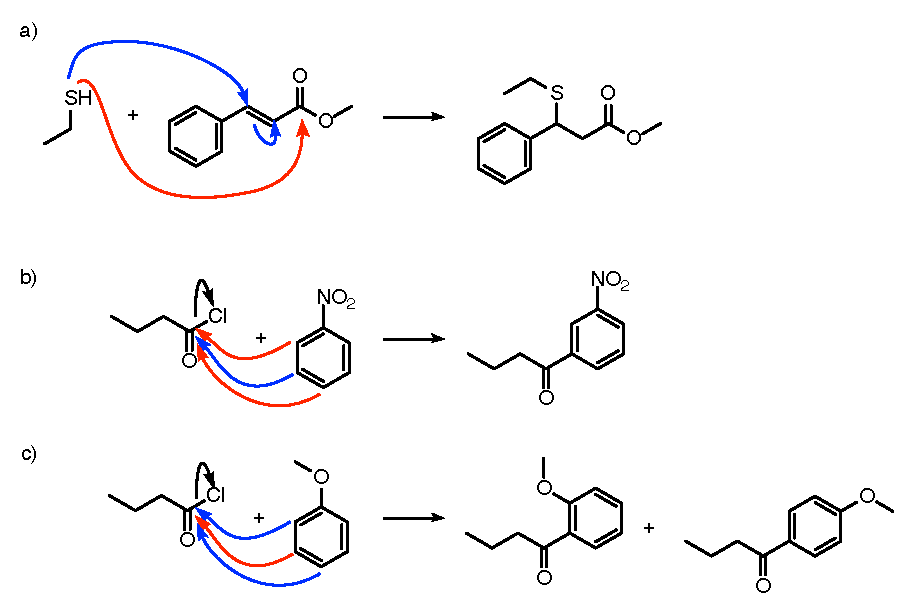
\includegraphics[width=0.7\textwidth]{imgs/textbook/additionalexamples.eps}
        \caption{Additional typical selectivity examples: Here, the expected product is shown on the right. The blue arrows indicate the top ranked paths from our model, the red arrows indicate other possibly competing but incorrect steps, which the model does not predict to be of high probability. In all cases, our model predicted the correct products. In b) and c), our model correctly recovers the regioselectivity expected in electrophilic aromatic substitutions.}
        \label{fig:extra-textbook-example2}
\end{figure*}





\end{document}
